Stablo valića je struktura koja iz ulaznog niza bitova gradi binarno stablo, gdje svaki čvor sadrži podniz početnog niza bitova \cite{grossi} \cite{bowe-th}. Navedenu strukturu su predložili Grossi, Gupta i Vitter \cite{bowe-th} u vidu predstavljanja jako dugih sekvenci i obavljanja brzih rang upita nad istima.

\section{Izgradnja stabla valića}

Za izgradnju stabla valića potrebno je za svaki čvor definirati abecedu ulaznog niza znakova, potom je potrebno abecedu podijeliti na dvije polovice te sve znakove ulaznog niza koji se nalaze u prvom dijelu abecede zamijeniti s 0, a ostale s 1. Obje polovice abecede se dalje dijele rekurzivno u djeci čvorovima sve dok nije moguće više podijeliti abecedu, to jest ostanu samo dva znaka u abecedi trenutnog čvora.

Algoritam dan pseudokom \ref{alg:wnode_construct} prikazuje postupak izgradnje stabla valića, te je na slici \ref{fig:wavelet_tree} prikazan primjer jednog tako izgrađenog stabla valića.

\begin{figure}[H]
	\centering
	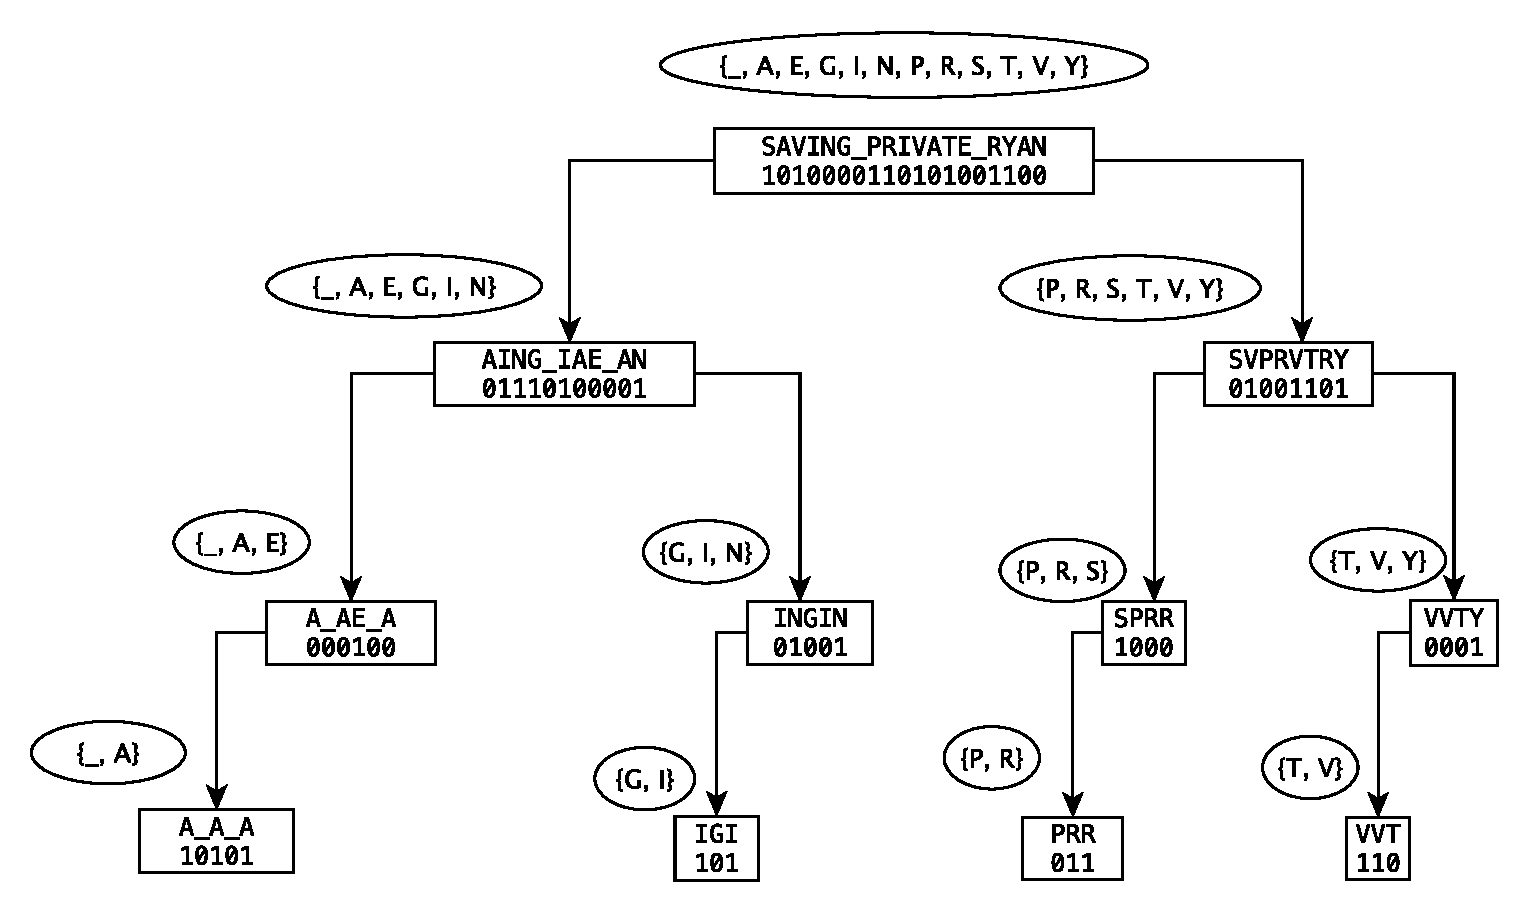
\includegraphics[width=0.9\textwidth]{img/wavelet_tree.pdf}
	\caption{Binarno stablo valića za niz \emph{Saving private Ryan}}
	\label{fig:wavelet_tree}
\end{figure}

\begin{algorithm}[H]
  \floatname{algorithm}{Pseudokod}
  \caption{Izgradnja čvora binarnog stabla valića, preuzeto iz \cite{breberic}}
  \begin{algorithmic}[1]
    \Function{izgradi}{$\Sigma, S$}
    \State Podijeli abecedu $\Sigma$ na dva jednaka dijela $\Sigma_1$ i $\Sigma_2$
    \State Kodiraj sve znakove $c \in \Sigma_1$ u nizu $S$ s 0, a ostale s 1
    \If{$|\Sigma_1| \geq S$}
      \State $S_1 \gets$ znakovi kodirani $0$ iz $S$ \State{}
      \Call{izgradi}{$\Sigma_1$, $S1$}
    \EndIf
    \If{$|\Sigma_2| \geq S$}
      \State $S_2 \gets$ znakovi kodirani $1$ iz $S$ \State{}
      \Call{izgradi}{$\Sigma_2$, $S2$}
    \EndIf
    \EndFunction
  \end{algorithmic}
  \label{alg:wnode_construct}
\end{algorithm}

\section{Upiti nad stablom valića}

Nad stablom valića definirani su sljedeći upiti:

\begin{itemize}
    \item $rank_c(i)$ - broj pojavljivanja znaka $c$ do pozicije $i$ u ulaznom nizu znakova
    \item $select_c(i)$ - pozicija $i$-tog znaka $c$ u ulaznom nizu znakova
    \item $access_c(i)$ - znak na $i$-toj poziciji u ulaznom nizu znakova
\end{itemize}

\subsection{\emph{Rank}}

\emph{Rank} upit za dani znak $c$ i poziciju $i$ ispituje koliko znakova $c$ se pojavljuje do pozicije $i$, uključeno s $i$-tom pozicijom. Algoritam je prikazan pseudokodom \ref{alg:wnode_rank}.

\begin{algorithm}[H]
  \floatname{algorithm}{Pseudokod}
  \caption{\emph{Rank} upit nad stablom valića, preuzeto iz \cite{breberic}}
  \begin{algorithmic}[1]
    \Function{rank}{$c, i$}
    \State $v \gets $ korijen stabla
    \State $r \gets i$
    \While{$v \neq null$}
      \If{$v \neq korijen$} \State $r \gets r - 1$ \EndIf
      \If{$c \in \Sigma_1$}
        \State $r \gets$ \Call{rank0}{$r$}
        \State $v \gets v_{lijevo}$
      \Else
        \State $r \gets$ \Call{rank1}{$r$}
        \State $v \gets v_{desno}$
      \EndIf
      \If{$r = 0$} \Return 0 \EndIf
    \EndWhile \State{}
    \Return $r$
    \EndFunction
  \end{algorithmic}
  \label{alg:wnode_rank}
\end{algorithm}

\subsection{\emph{Select}}

\emph{Select} upit za dani znak $c$ i broja pojavljivanja znaka tog znaka $i$ ispituje na kojoj poziciji se nalazi $i$-ti znak $c$. Algoritam je prikazan pseudokodom \ref{alg:wnode_select}.

\begin{algorithm}[H]
  \floatname{algorithm}{Pseudokod}
  \caption{\emph{Select} upit nad stablom valića, preuzeto iz \cite{breberic}}
  \begin{algorithmic}[1]
    \Function{select}{$c, i$}
    \State $v \gets $ čvor koji predstavlja znak $c$
    \State $r \gets i$
    \If{$c \in \Sigma_1$}
      \State $r \gets $ \Call{select0$_v$}{$r$}
    \Else
      \State $r \gets $ \Call{select1$_v$}{$r$}
    \EndIf
    \While{$v \neq $ korijen}
      \State $r \gets r + 1$
      \State $p \gets $ \Call{roditelj}{v}
      \If{$v$ lijevo dijete od $p$}
        \State $r \gets $ \Call{select0$_p$}{$r$}
      \Else
        \State $r \gets $ \Call{select1$_p$}{$r$}
      \EndIf
      \State $v \gets p$ 
    \EndWhile \State{}
    \Return $r$
    \EndFunction
  \end{algorithmic}
  \label{alg:wnode_select}
\end{algorithm}

\subsection{\emph{Access}}

\emph{Access} upit za danu pozicijiu $i$ vraća $i$-ti znak sekvence. Algoritam je prikazan pseudokodom \ref{alg:wnode_access}.

\begin{algorithm}[H]
  \floatname{algorithm}{Pseudokod}
  \caption{\emph{Access} upit nad stablom valića, preuzeto iz \cite{breberic}}
  \begin{algorithmic}[1]
    \Function{Access}{$i$}
    \State $v \gets $ korijen stabla
    \State $r \gets i$
    \While{$v \neq null$}
      \If{$v \neq korijen$} \State $r \gets r - 1$ \EndIf
      \If{\Call{access}{r} $= 0$}
        \State $r \gets $ \Call{rank0}{$r$}
        \If{$v_{lijevo} = null$} \Return prvi znak iz $\Sigma_v$ \EndIf
        \State $v \gets v_{lijevo}$
      \Else
        \State $r \gets $ \Call{rank1}{$r$}
        \If{$v_{desno} = null$} \Return zadnji znak iz $\Sigma_v$ \EndIf
        \State $v \gets v_{desno}$
      \EndIf
    \EndWhile\State{}
    \Return $r$
    \EndFunction
  \end{algorithmic}
  \label{alg:wnode_access}
\end{algorithm}
